\documentclass[12pt]{article}
\usepackage{sbc-template}
\usepackage{graphicx,url}
\usepackage[brazil]{babel}   
\usepackage[utf8]{inputenc}  
\usepackage{float}
\usepackage{textcomp}
\usepackage[table,xcdraw]{xcolor}

%-------------- APENAS PARA UBUNTU 16 ----------------
%Este trecho foi inserido por conta de um bug presente
%no Ubuntu 16.04 no qual não mostra os índices das sessões

\usepackage{etoolbox}
\makeatletter
\patchcmd{\ttlh@hang}{\parindent\z@}{\parindent\z@\leavevmode}{}{}
\patchcmd{\ttlh@hang}{\noindent}{}{}{}
\makeatother
%------------------------------------------------------    

\sloppy

\title{Estudo de Algoritmos de Previsão de Desvio\\com o Simulador Gem5}

\author{Leonardo Vendrame\inst{1}}

\address{Departamento de Informática -- Universidade Estadual de Maringá (UEM)\\
  Maringá -- PR -- Brasil
\email{leonvendrame@gmail.com}
}

\begin{document} 

\maketitle

\begin{abstract}
  This paper presents a study about branch prediction. Branch prediction aims to improve the performance
  of applications execution, but, there's several algorithms to do it, that may have different performances.
  The objetivo is to look for the best-case branch prediction algorithm to the largest applications domain.
  Inside the study's scope, the LTAGE algorithm was the one who demonstrated the best results.
\end{abstract}
     
\begin{resumo} 
  Este \textit{paper} apresenta um estudo sobre previsão de desvio. Previsão de desvio visa melhorar
  o desempenho de execução de aplicações, porém, existem diversos algoritmos para isso, que podem
  ter desempenhos diferentes. O objetivo é buscar o algoritmo de previsão de desvio que se sai melhor para
  o maior domínio de aplicações. Dentro do escopo do estudo o algoritmo LTAGE foi o que demonstrou os
  melhores resultados.
\end{resumo}


\section{Introdução}

O desempenho da execução real de um programa pode ser medido de diversas formas,
visto que é possível tomar como base vários aspectos. Tomando como foco o tempo de execução, é possível
realizar a análise detalhada de processamento, procurando eliminar desperdícios de tempo.

Para que se obtenha um menor tempo de execução, é importante que o \textit{pipeline} dos processadores esteja 
sempre completo, procurando impedir que existam ciclos de \textit{clock} em que o processador fique ocioso. 
Porém, existem determinados problemas que podem impedir que o \textit{pipeline} continue completo, 
um destes problemas é o de saltos. 

Saltos são, resumidamente, instruções que permitem saltar para determinados trechos de
código do programa. Existem saltos incondicionais e saltos condicionais. O primeiro não gera
problema dentro de um \textit{pipeline}, visto que deverá ser tomado, e portanto as próximas
instruções devem ser aquelas imediatamente depois do salto. Porém, saltos condicionais podem
gerar problemas. Um salto condicional, deverá ser tomado ou não somente após a execução de sua condição,
o que acontece somente alguns estágios após a etapa de busca das próximas instruções. Com isso,
pode ocorrer a busca de operações que não deveriam ser executadas, ocasionando numa perda de ciclos
de \textit{clock} úteis para processamento.

Visando diminuir ao máximo essa perda, foram desenvolvidos
os algoritmos de previsão de desvio, ou, a téncica de execução especulativa \cite{pedronette:06},
isto é, algoritmos que tentam prever o comportamento do salto, especulando se este deve ou não ser tomado
antes mesmo da execução de sua condição, procurando assim, buscar pelas próximas instruções que realmente
deveriam ser executadas. 

\section{O Simulador Gem5} \label{simg5}

O Simulador Gem5 é uma união da infraestrutura de dois simuladores conhecidos como \textit{M5} e \textit{GEMS}. 
Com isso o Gem5 fornece um ambiente de simulação com uma ampla capacidade de configuração, oferencendo diversas
arquiteturas de conjuntos de instruções, bem como diversos modelos de processadores, aliados à um sistema de memória
com suporte a múltiplas caches \cite{gem5sim}.

Simuladores como este dão base à pesquisas, testes e até mesmo projeções de produtos que podem vir a serem desenvolvidos.
Fornecendo uma gama de recursos e permitindo a customização de uma arquitetura, o Gem5 permite um estudo sobre o
comportamento dos algoritmos de previsão de desvio. Além da escolha do modelo de processador é possível também definir 
suas propriedades, entre elas, o aspecto aqui desejado, algoritmo de previsão de desvio. A partir disso o simulador
se torna uma ferramenta capaz de prover informações específicas sobre tais algoritmos, fornecendo os dados resultantes 
de suas simulações, dando a possibilidade de que um algoritmo específico seja testado para diversos programas de entrada.

O simulador possui dois modos de execução, o \textit{SE (System-call Emulation)} que captura e emula todas as chamadas
ao sistema, e o \textit{FS (Full-System)} que simula um sistema completo, provendo um ambiente de simulação baseado em um
sistema operacional.

O Gem5 pode simular as seguintes arquiteturas: \textit{ARM}, \textit{ALPHA}, \textit{MIPS}, \textit{Power}, \textit{SPARC}, e \textit{x86}.
Sendo que as arquiteturas \textit{ARM}, \textit{ALPHA}, e \textit{x86} incluem suporte ao \textit{boot} ao \textit{Linux}.

\section{Algoritmos de Previsão de Desvios}

Algoritmos de previsão de desvio, são algoritmos que visam prever o comportamentos de instruções de saltos dentro de uma
aplicação. O objetivo dessa especulação é ganhar desempenho, buscando amenizar que o processador faça trabalho que não será
usado, isto é, processe informações que serão descartadas após seu processamento ao invés de serem efetivadas. 

A execução especulativa de instruções permite aos processadores ganharem tempo eliminando instruções inúteis, porém, isso só 
acontece caso a especulação seja tomada corretamente. Nos casos de erro de especulação, o processador já terá buscado outras 
instruções, pois o mesmo só saberá que a especulação foi incorreta durante a execução da condição do salto. As instruções que
foram buscadas especulativamente serão executadas antes que o processador possa buscar as instruções corretas, e neste caso os resultados
das mesmas não serão efetivados, portanto, descartados.
Neste tempo o processador gastou ciclos de clock com processamento desnecessário.

Algoritmos de previsão de desvio com alta precisão são essenciais em \textit{pipelines} muito profundos e são um fator de extrema
importância em processadores superescalares \cite{evers:96}, visto que, deseja-se
obter resultados no menor tempo possível e sempre minimizar o desperdício de ciclos de \textit{clock}. Em média, a cada cinco
instruções, uma é operação de desvio \cite{nicacio:06}, portanto, mostram-se necessários algoritmos com taxas de acerto cada
vez maiores.

Existem algoritmos de previsão estática e algoritmos de previsão dinâmica. Algorimos de previsão estática tomam sempre um determinado
comportamento, como por exemplo tomar todos os saltos, ou não tomar nenhum salto. Já algoritmos dinâmicos possuem comportamentos
variados e tentam analisar das mais diversas maneiras se um salto deve ou não ser tomado, isso acontece durante a execução da aplicação.
Destacam-se alguns algoritmos de previsão dinâmica:

\begin{description}
\item \textbf{\textit{LTAGE}}: É um preditor de desvio baseado em histórico global. Apresenta um preditor bimodal indexado por \textit{PC} (\textit{Program Counter)} 
e N tabelas parcialmente demarcadas, indexadas com um \textit{hash} de \textit{PC} e do histórico global de predição. Todas as suas tabelas são acessadas
paralelamente e aquela usando o maior histórico que combina é a que dá a predição (com algumas exceções). Além disso ainda conta com um preditor de 
\textit{loops} que guarda o contador de interações de \textit{loops} e os prevê de acordo.

\item \textbf{\textit{BiMode}}: É um preditor de dois níveis que possui três vetores de histórico separados: um de saltos tomados, um de saltos não tomados e um 
de escolha. Visa eliminar o \textit{aliasing} destrutivo que ocorre quando duas predições diferentes compartilham o mesmo padrão de histórico global, e 
faz isso por separar as predições em vetores separados de saltos tomados e não tomados e usando o desvio do \textit{PC} (\textit{Program Counter}) para escolher 
entre eles dois.

\item \textbf{\textit{Tournament}}: Também conhecido como híbrido, o algoritmo Tournament geralmente combina o funcionamento dois algoritmos
de previsão, tentando se adequar às diferentes aplicações que possam vir a serem executadas.

\item \textbf{\textit{Local (2 Bits)}}: Consiste de utilizar 2 bits para prever o desvio, um bit diz se deve ou não ser tomado e o outro diz se
o preditor acertou ou não a ultima previsão. Geralmente é implementado através de um somador saturado.
\end{description}

\section{Experimentos e Discussão}
Serão apresentados aqui informações sobre os experimentos e resultados obtidos, bem como questões observadas na realização
do projeto.

\subsection{Ambiente de Testes}

\begin{description}
\item \textbf{\textit{Hardware:}} Para a simulação foi utillizado um dispositivo com as seguintes características: \\
Processador: Intel\textsuperscript\textregistered  Xeon\textsuperscript\textregistered  CPU @ 2.20GHz.\\
Memória RAM: 8GB.\\
Sistema Operacional: Debian 9.4 (Stretch) 64 Bits.\\
Disco Rígido: SSD 20GB.\\

\item \textbf{\textit{Software:}} A execução se deu através do Gem5 com uma arquitetura simulada com as seguintes características:\\
Gem5: Modo \textit{SE (System-call Emulation)}. Versão \textit{gem5.fast 2.0}.\\
Processador: O3CPU @ 2GHz.\\
Conjunto de Instruções: x86.\\
Cache: Multi-nível de 2 níveis.\\
Cache L1: Dividida entre dados e instruções. L1D: 16KB e L1I: 64KB.\\
Cache L2: Unificada. L2: 256KB.\\
Memória RAM: 3GB\\
Compilador: \textit{GCC 6.3.0}.

\item \textbf{\textit{Algoritmos e Aplicações:}} Algoritmos e aplicações simulados:\\
Algoritmos de previsão: \textit{LTAGE}, \textit{BiMode}, \textit{Local (2 Bits)} e \textit{Tournament}. 
Aplicações: \textit{nbench (LLVM test-suite)}, \textit{dijkstra (Polybench)}, \textit{floyd-warshall (CBench)}, \textit{flops-8 (LLVM test-suite)} 
e \textit{mpeg2enc (MediaBench II)}. 

%%\begin{description}
 \textbf{\textit{nbench:}} Aplicação de Benchmark.\\
 \textbf{\textit{dijkstra:}} Determina o caminho mínimo, partindo de um vértice de início v para todos os outros vértices do grafo.\\
 \textbf{\textit{floyd-warshall:}} Determina a distância entre todos os pares de vértices de um grafo.\\
 \textbf{\textit{flops-8:}} Procura estimar a taxa de MFlops do sistema para determinadas operações baseadas em um mix de instruções específicas.\\
 \textbf{\textit{mpeg2enc:}} Codifica diversos arquivos \textit{.ppm (Netpbm color image format)} em um arquivo \textit{.mpg}.\\

%%\end{description}
\end{description}

% Além disso, o simulador Gem5 foi compilado no modo \textit{fast} para uma arquitetura com conjunto de instruções \textit{x86}
% e foi executado no modo \textit{SE (System-call Emulation)}, isto é, ele captura e emula as chamadas ao sistema.
% como o processador O3CPU com \textit{clock} de 2GHz, memória RAM de 3GB e um arquivo \textit{caches.py} com as configurações
% de uma cache multi-nível de 2 níveis, sendo o primeiro nível separado em cache de instruções (64KB) e de informações
% \textit{(data)} (16KB) e o segundo nível unificado (256KB). 

% % Os algoritmos de previsão de desvio testados foram: 

% As aplicações utilizadas para testes foram: 

\subsection{Metodologia e Experimentos}

Todos os algoritmos foram compilados utilizando a flag de otimização \textit{-O3}. 

Após compiladas, cada aplicação é executada uma vez para cada algoritmo de previsão de desvio. Desta forma, é possível obter
o desempenho de cada algoritmo em situações e domínios variados.

Uma vez executadas as aplicações, o ambiente Gem5 gera um arquivo contendo todas as informações daquela execução, 
permitindo obter detalhes dos mais diversos aspectos. Aqui serão analisados os aspectos referentes a previsão de
desvio, com foco na quantidade de erros e acertos, a fim de expor situações em que os algotimos podem ser mais eficientes.

Analisando as estatísticas presentes no final das simulações é possível obter o número de predições totais e incorretas de cada 
algoritmo para cada aplicação, resultando nas taxas de erros e acertos que serão avaliadas e apresentadas, com o objetivo de mostrar
dados palpáveis da eficácia de tais algoritmos.

\subsection{Questões}
Destacam-se algumas questões a serem respondidas com a execução dos experimentos:\\
Qual é a taxa de acerto de cada algoritmo? Qual algoritmo se sai melhor no geral?\\
Qual é a taxa de erro de cada algoritmo? Qual algoritmo se sai pior no geral?\\
O domínio de aplicação e a aplicação em si influenciam nos resultados? De que maneira?

\subsection{Resultados}

Visando responder as questões apresentadas acima, temos os resultados a seguir.

\begin{figure}[H]
\centering
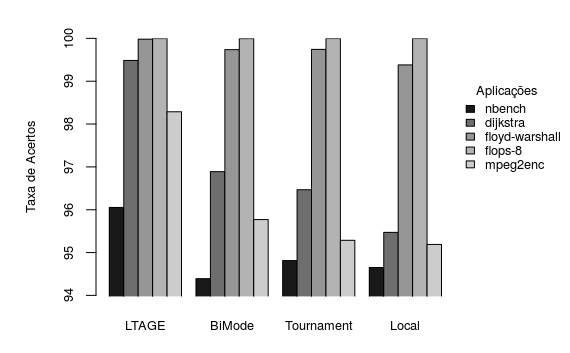
\includegraphics[width=0.66\textwidth]{algTax.jpeg}
\caption{Resultado: Taxa de Acertos por Algoritmo}
\label{fig:algTax}
\end{figure}

Através da Figura \ref{fig:algTax} pode-se observar a taxa de acerto de cada algoritmo de previsão de desvio. A média
da taxa de acerto geral do escopo do projeto foi de 97.57\%. Isso pode ser considerado uma boa taxa de acertos, porém, fora
do escopo do projeto os processadores precisam lidar com um número expressivamente maior de domínios de aplicações, o que faz
com que na prática, nem sempre os algoritmos de previsão de desvio alcancem tais taxas.

Fica exposto que em todos os casos, salvo à exceção de empate de performance na execução da aplicação \textit{flops-8},
o algoritmo \textit{LTAGE} foi o que obteve a maior taxa de acerto. Além disso, pode-se também notar um padrão quando se olha
para todos os algoritmos, de maneira geral, as barras se comportam de maneiras semelhantes. De maneira complementar à Figura \ref{fig:algTax}
é possível se obter também as taxas de erros dos algoritmos em questão, que variam entre 0,004\% e 5,608\%, com média de 2,42\%. %%No outro trabalho a informação estava equivocada.
Para terminar de responder às primeiras questões, o algoritmo que se saiu pior no geral foi o \textit{Local (2 Bits)}, que 
conseguiu as menores taxas de acertos em 80\% dos casos.

Procurando dar resposta à última questão, vamos organizar os dados de uma forma diferente, verificando os resultados desta vez
por aplicação.

\begin{figure}[H]
\centering
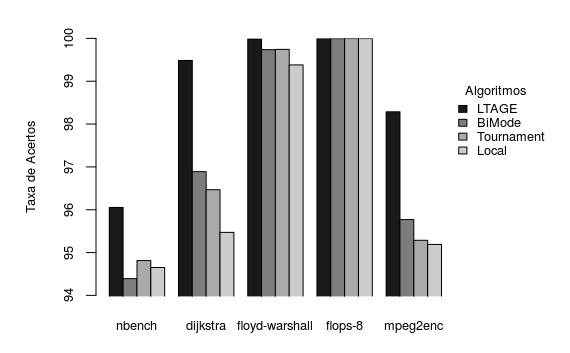
\includegraphics[width=0.66\textwidth]{appTax.jpeg}
\caption{Resultado: Taxa de Acertos por Aplicação}
\label{fig:appTax}
\end{figure}

Com a nova organização da Figura \ref{fig:appTax}, evidenciamos que as aplicações e seus domínios influenciam no resultado dos algoritmos
de previsão de desvio, isto é, existem certas aplicações que vão obter melhores resultados que outras. Um exemplo disso é 
a aplicação \textit{flops-8}, que garantiu uma taxa de acertos maior que quaisquer outras.

Os preditores se mostraram no geral eficazes e precisos nos testes realizados, com taxas de acertos acima de 94\%. Entretando ainda houve 
certa diferença. Analisando a aplicação \textit{flops-8}, ela basicamente não lida com instruções condicionais do tipo \textit{if},
mas sim com \textit{loops} do tipo \textit{for}. Isto pode explicar as predições próximas de 100\%, visto que até mesmo em um algoritmo de 
previsão local com um histórico de 2 bits seriam poucas as vezes em que o algoritmo erraria a predição, basicamente na entrada 
e na saída do \textit{loop}. Diferentemente da aplicação \textit{nbench} que demonstra a menor média de acerto, com cerca de 95\% e possui 
diversos casos condicionais tanto de instruções do tipo \textit{if}, quanto de instruções do tipo \textit{case} dentro de \textit{switches}.

Portanto, quanto maior for o índice de condicionais maiores são as chances da especulação ser errada, o que expõe que os algoritmos
de previsão de desvio se saem melhor com casos de \textit{loops} e aplicações simplesmente iterativas ao invés de aplicações em que a entrada
é imprevista e pode dividir o fluxo de instruções em muitas partes, com muitas instruções condicionais.

\section{Conclusão}

Algoritmos de previsão de desvio possuem grande importância no desempenho da execução 
de programas dentro de um processador, eles ditam o desempenho e o número de ciclos úteis quando
instruções são executadas especulativamente. Portanto, quanto melhor o algoritmo, isto é, quanto menor for 
a taxa de erro do mesmo, menos tempo é desperdiçado com instruções que não deveriam ser executadas.

Apesar da grande eficácia atual de tais algorítmos eles ainda não são perfeitos e falham em conseguir 
prever todas as especulações. Desta forma, ainda existem instruções que são processadas sem que seus
resultados sejam efetivamente úteis para as aplicações.

Contudo, a taxa de acertos, como mostrada durante os testes realizados, pode se mostrar muito próxima de 100\% em algoritmos com poucas instruções
condicionais. Além disso existem algoritmos que se saem melhor para determinadas aplicações. 

Com os testes demonstra-se a importância de um estudo mais aprofundado e detalhado antes da implementação de algoritmos de previsão de desvio em \textit{hardware},
visto que depois de implementados os mesmos não podem ser alterados tão facilmente quanto via \textit{software} e portanto, deve-se procurar encontrar o que ofereça 
o melhor desempenho para os mais amplos de domínios de aplicações.

\bibliographystyle{sbc}
\bibliography{sbc-template}

\end{document}